\chapter{Résultats} \label{Resultats}

\section{Planning final }

Le diagramme de Gantt (cf. \ref{GanttFinal}) montre le planning final de mon stage. Contrairement au planning élaboré en début de stage, la chaîne de traitements était déjà opérationnel au bout de quatre mois de travail et nous avons pu réadapter nos objectifs et développer en plus un logiciel ouvert.

\begin{center}
\begin{figure}[h] \centering
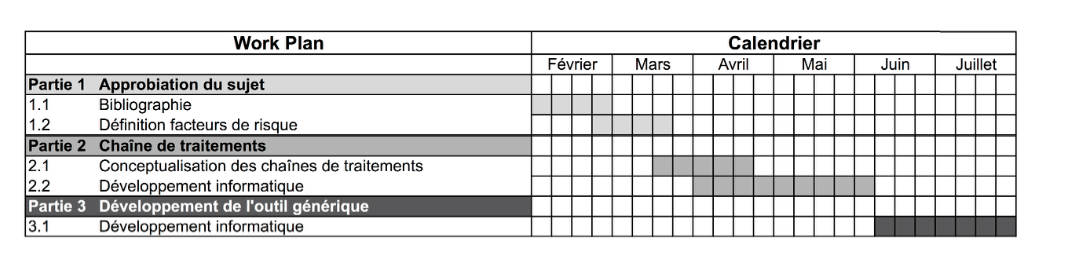
\includegraphics[width=14cm]{GanttFinal}\\
\caption{\label{GanttFinal} Planning final }
\end{figure}
\end{center}

\section{Prototype }

Nous avons développé deux outils, basés sur des plateformes Open Source. Le premier outil, une chaîne de traitements automatisée fermée qui permet d'effectuer des traitements dans un ordre bien défini pour cartographier des indicateurs de risque environnemental. Le deuxième outil, un \textbf{logiciel ouvert}, donne à l'utilisateur la possibilité d'exécuter et de combiner chacun des traitements de la chaîne selon  ses besoins. 

\begin{center}
\begin{figure}[h] \centering
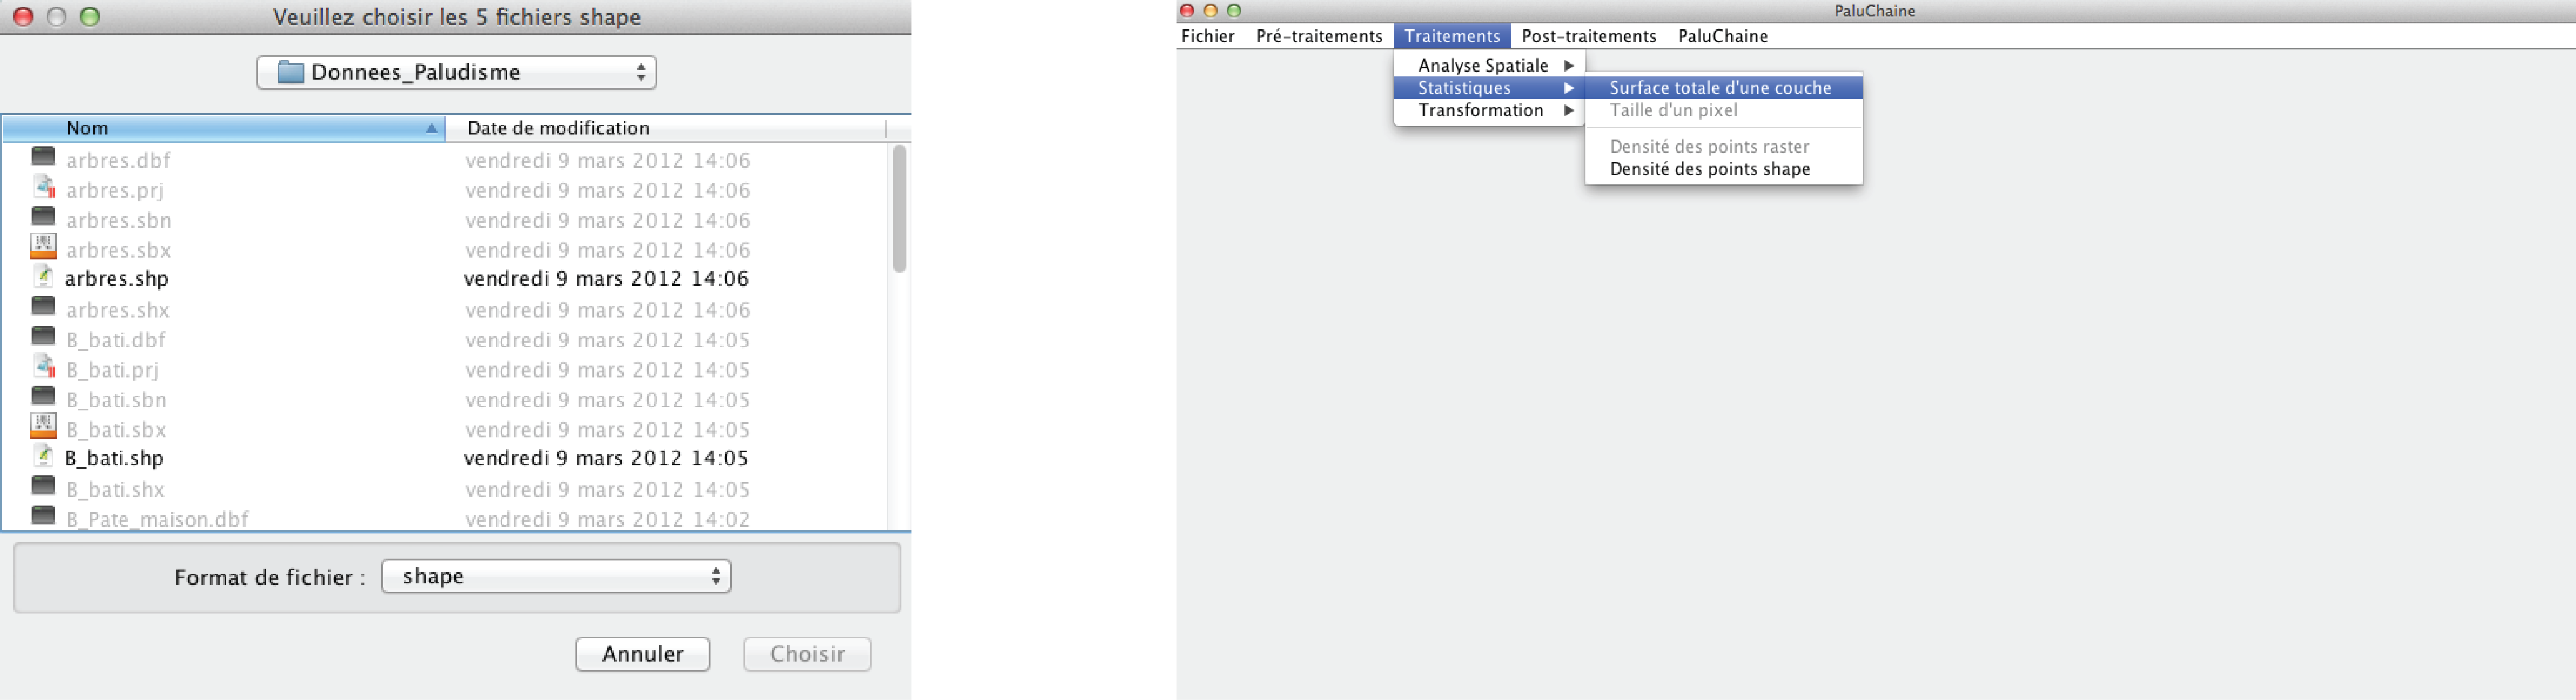
\includegraphics[width=14cm]{Results}\\
\caption{\label{Results} Aperçus des deux outils ("ouvert à droite) }
\end{figure}
\end{center}

\section{Validation des résultats}

Pour valider les résultats et surtout le fonctionnement de la chaîne de traitements, nous comparons une carte de vulnérabilité, une carte d'aléa et une carte de risque créées par la chaîne aux cartes de risque élaborée par Nadine Dessay en utilisant le logiciel ArcGIS.

\paragraph{Comparaison cartes de vulnérabilité\\\\}

\begin{center}
\begin{figure}[h] \centering
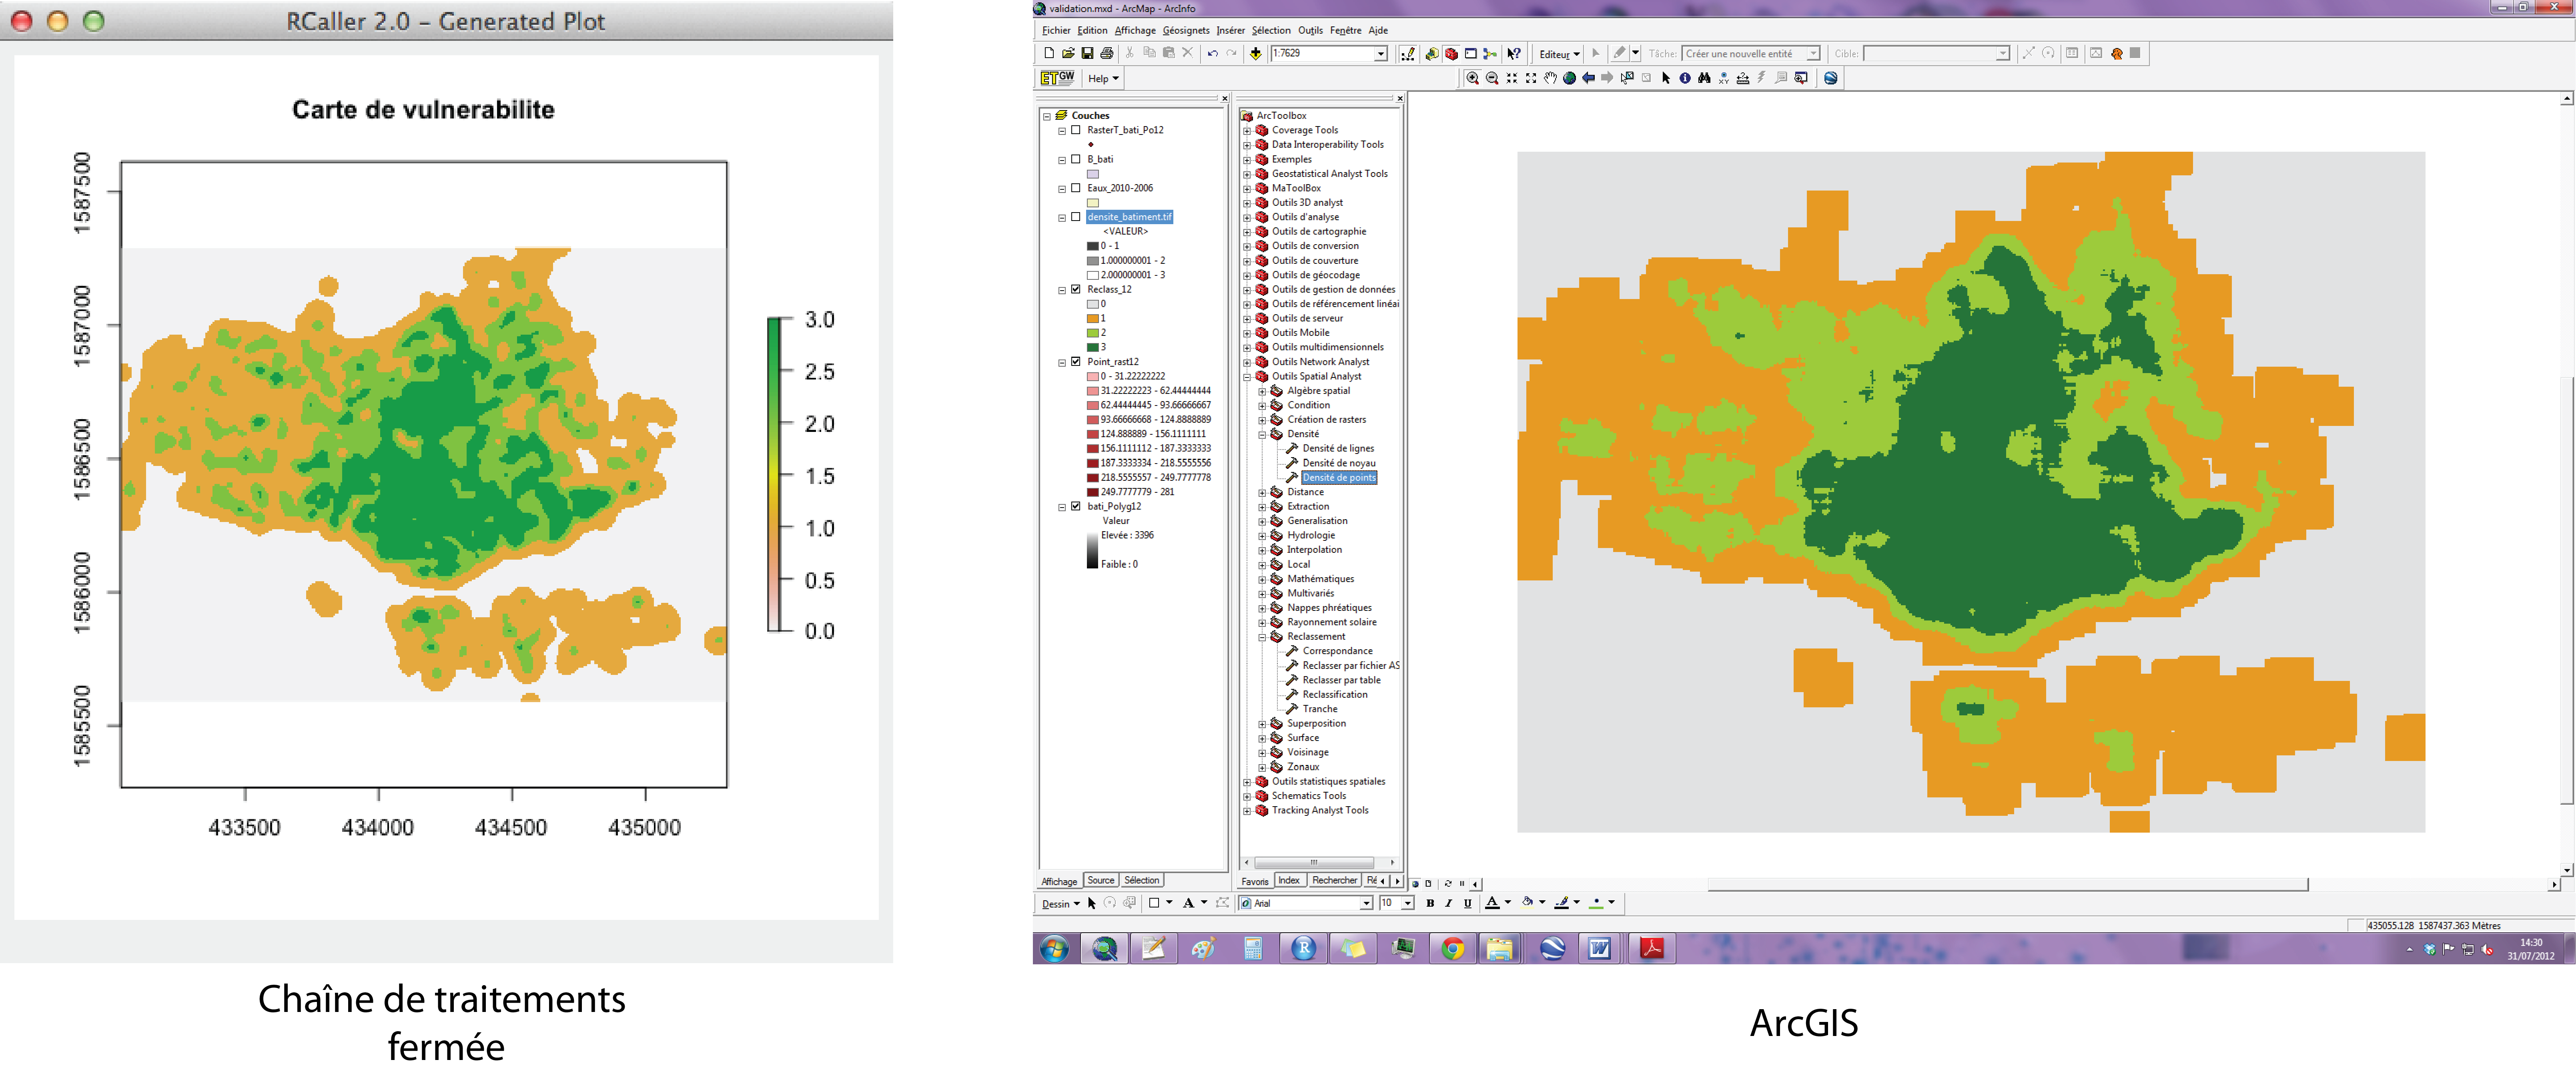
\includegraphics[width=14cm]{VulerabiliteComp}\\
\caption{\label{VulnerabComp} Cartes de vulnérabilté }
\end{figure}
\end{center}

Les deux cartes se ressemblent fortement. En analysant les statistiques des deux images raster générées, nous pouvons nous apercevoir que les résultats sont très similaires. \\
La carte générée à partir de la chaîne de traitements fermée présente les résultats suivants:
\begin{itemize}

\item Moyenne: 0.855 (valeur moyenne des cellules)
\item Ecart-type: 1.0249 (Ecart-type des cellules de l'image)\\

\end{itemize} 

La carte générée avec l'outil ArcGIS présente les résultats suivants:

\begin{itemize}

\item Moyenne: 0.9287 (valeur moyenne des cellules)
\item Ecart-type: 1.0461 (Ecart-type des cellules de l'image)\\

\end{itemize} 

Les différences entre les deux cartes sont donc minimes et comme l'aperçu des deux cartes est également très similaire nous pouvons donc valider le résultat de la carte de vulnérabilité.\\

Les petites différences peuvent être expliquées par le fait que ArcGIS et R (utilisé pour les calculs statistiques dans la chaîne de traitements fermée) utilisent des algorithmes différents pour effectuer les différentes calculs. Par exemple, lors du calcul de la densité des points, sous ArcgIS on a la possibilité de choisir entre plusieurs types de voisinage (rectangulaire, circulaire...). Nadine Dessay utilise le voisinage rectangulaire pour son travail. R et plus précisément le package "raster" utilise par défault un voisinage circulaire ce qui fait qu'en sortie les pixels des deux cartes ne sont pas identiques (rectangulaire sous ArcGIS et circulaire sous R).


\paragraph{Carte d'aléa\\\\}

\begin{center}
\begin{figure}[h] \centering
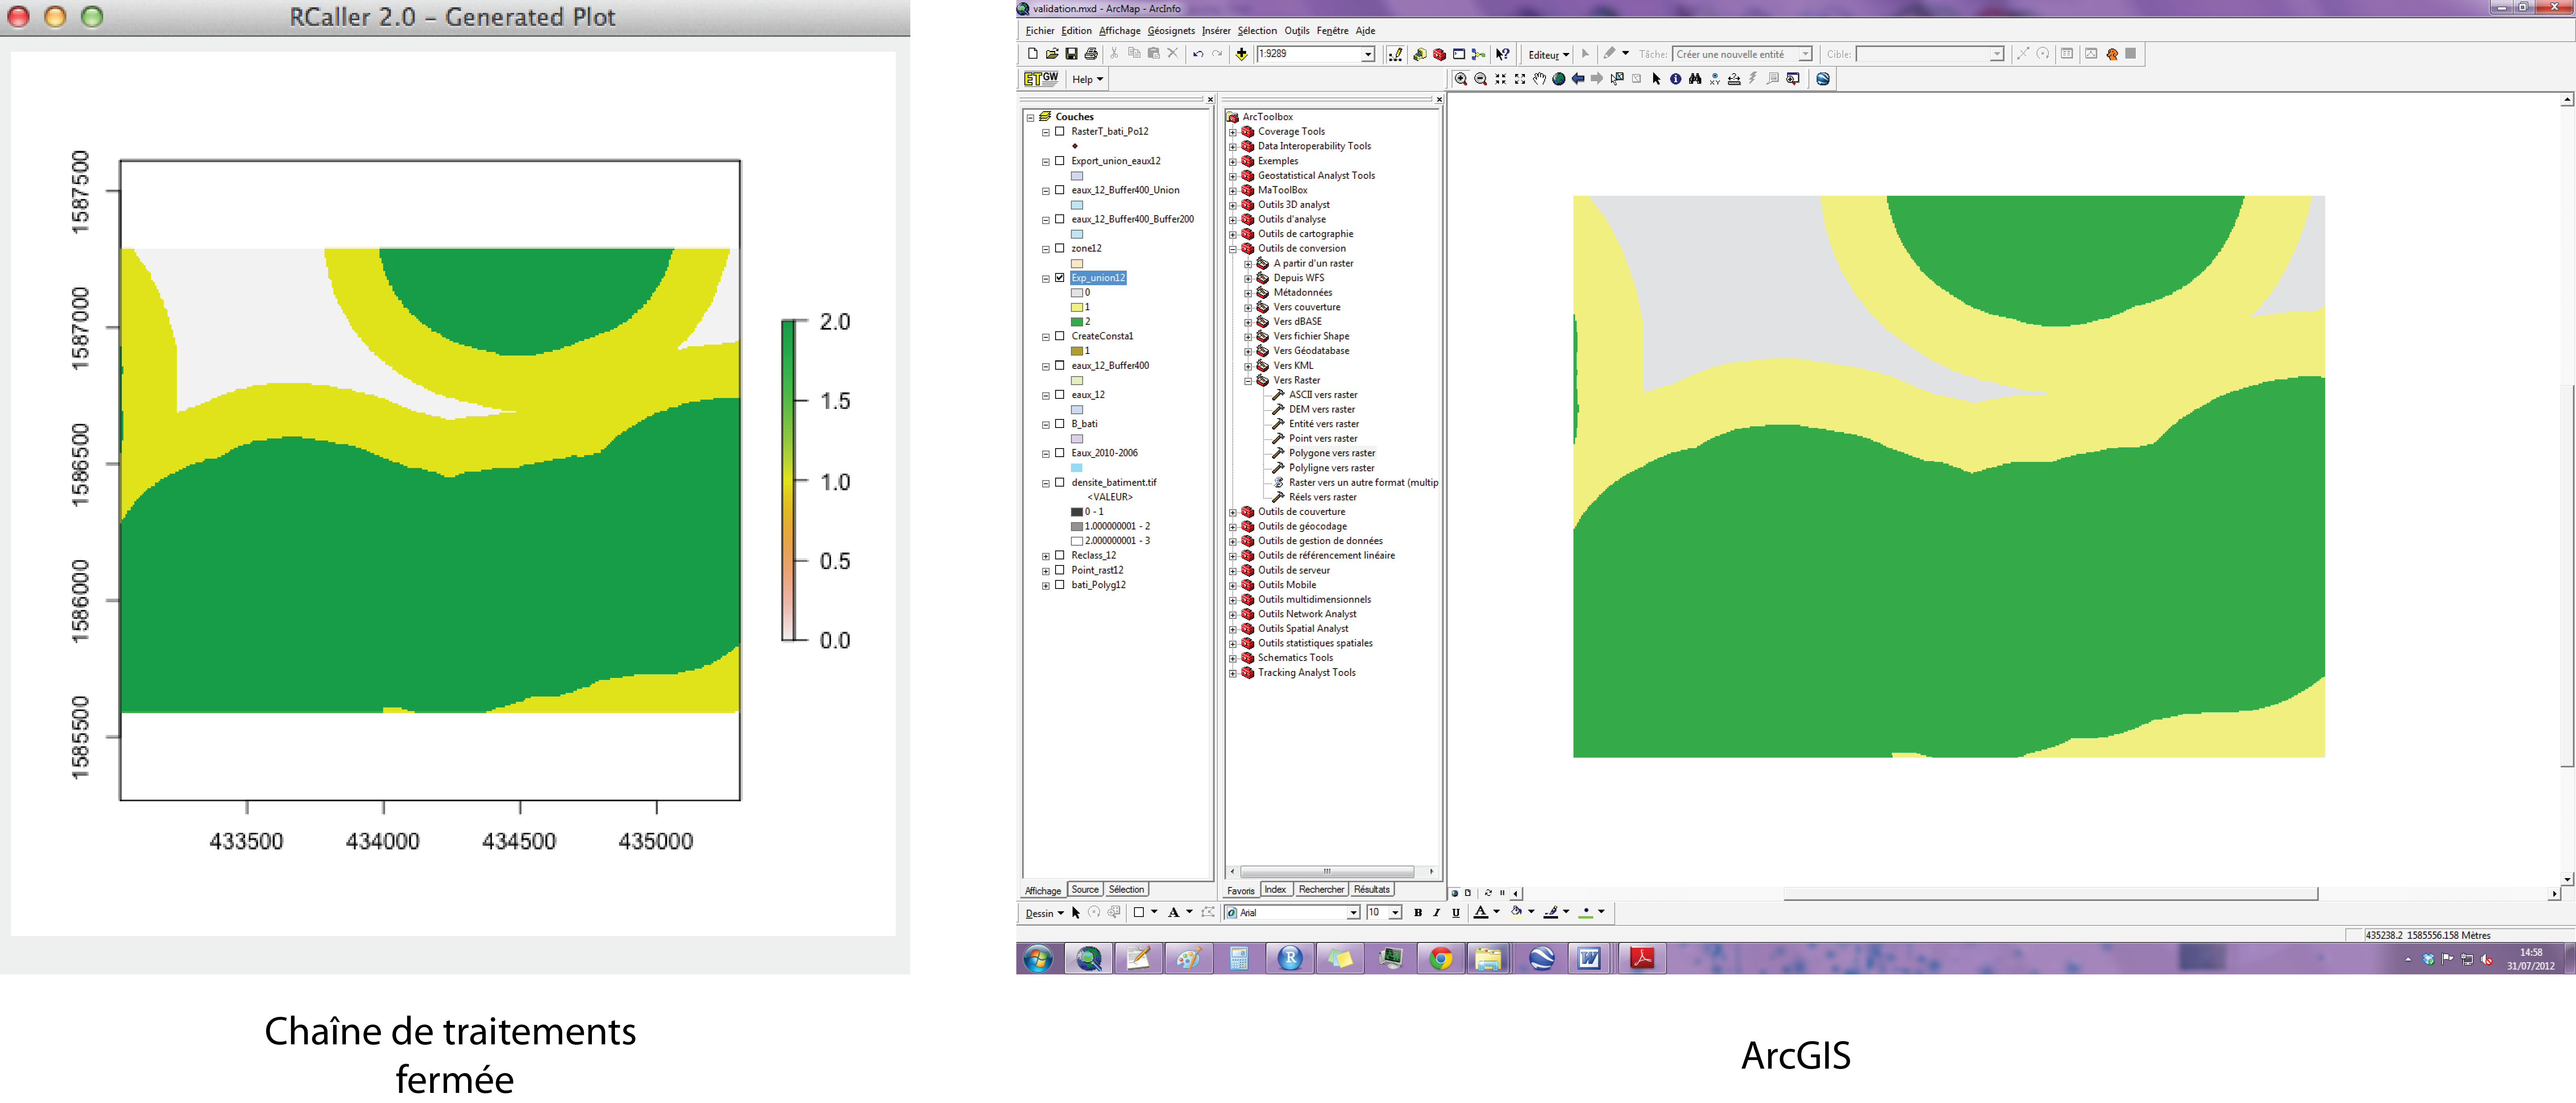
\includegraphics[width=14cm]{AleaComp}\\
\caption{\label{AleaComp} CArtes d'aléa}
\end{figure}
\end{center}

Pour l'élaboration de cette carte nous créons 2\textbf{ zones tampons} différentes: \\

Une zone tampon de 400 mètres autour des surfaces aquatiques. Sous ArcGIS, il existe la possibilité de créer par la suite une deuxième zone tampon autour de cette nouvelle couche créé (zones tampon de 400 mètres), dans notre cas de 200 m.\\
A l'intérieur de la chaîne de traitements cette opération est effectuée de la manière suivante: Création d'une zone tampon de 400 mètres et création d'une zone tampon de 600 mètres autour des surfaces aquatiques. \\
Par la suite nous créons une nouvelle donnée en soustrayant ces deux couches. Nous obtenons donc une couche correspondant à la zone tampon (200 mètres) autour de la zone de tampon de 400 mètres. \\
Comme on peut s'apercevoir en comparant les deux cartes (cf. \ref{AleaComp}), les résultats sont tout à fait identiques et nous pouvons valider le résultat de la chaîne de traitements fermée concernant la carte d'aléa.

\paragraph{Carte de risque\\\\}

\begin{center}
\begin{figure}[h] \centering
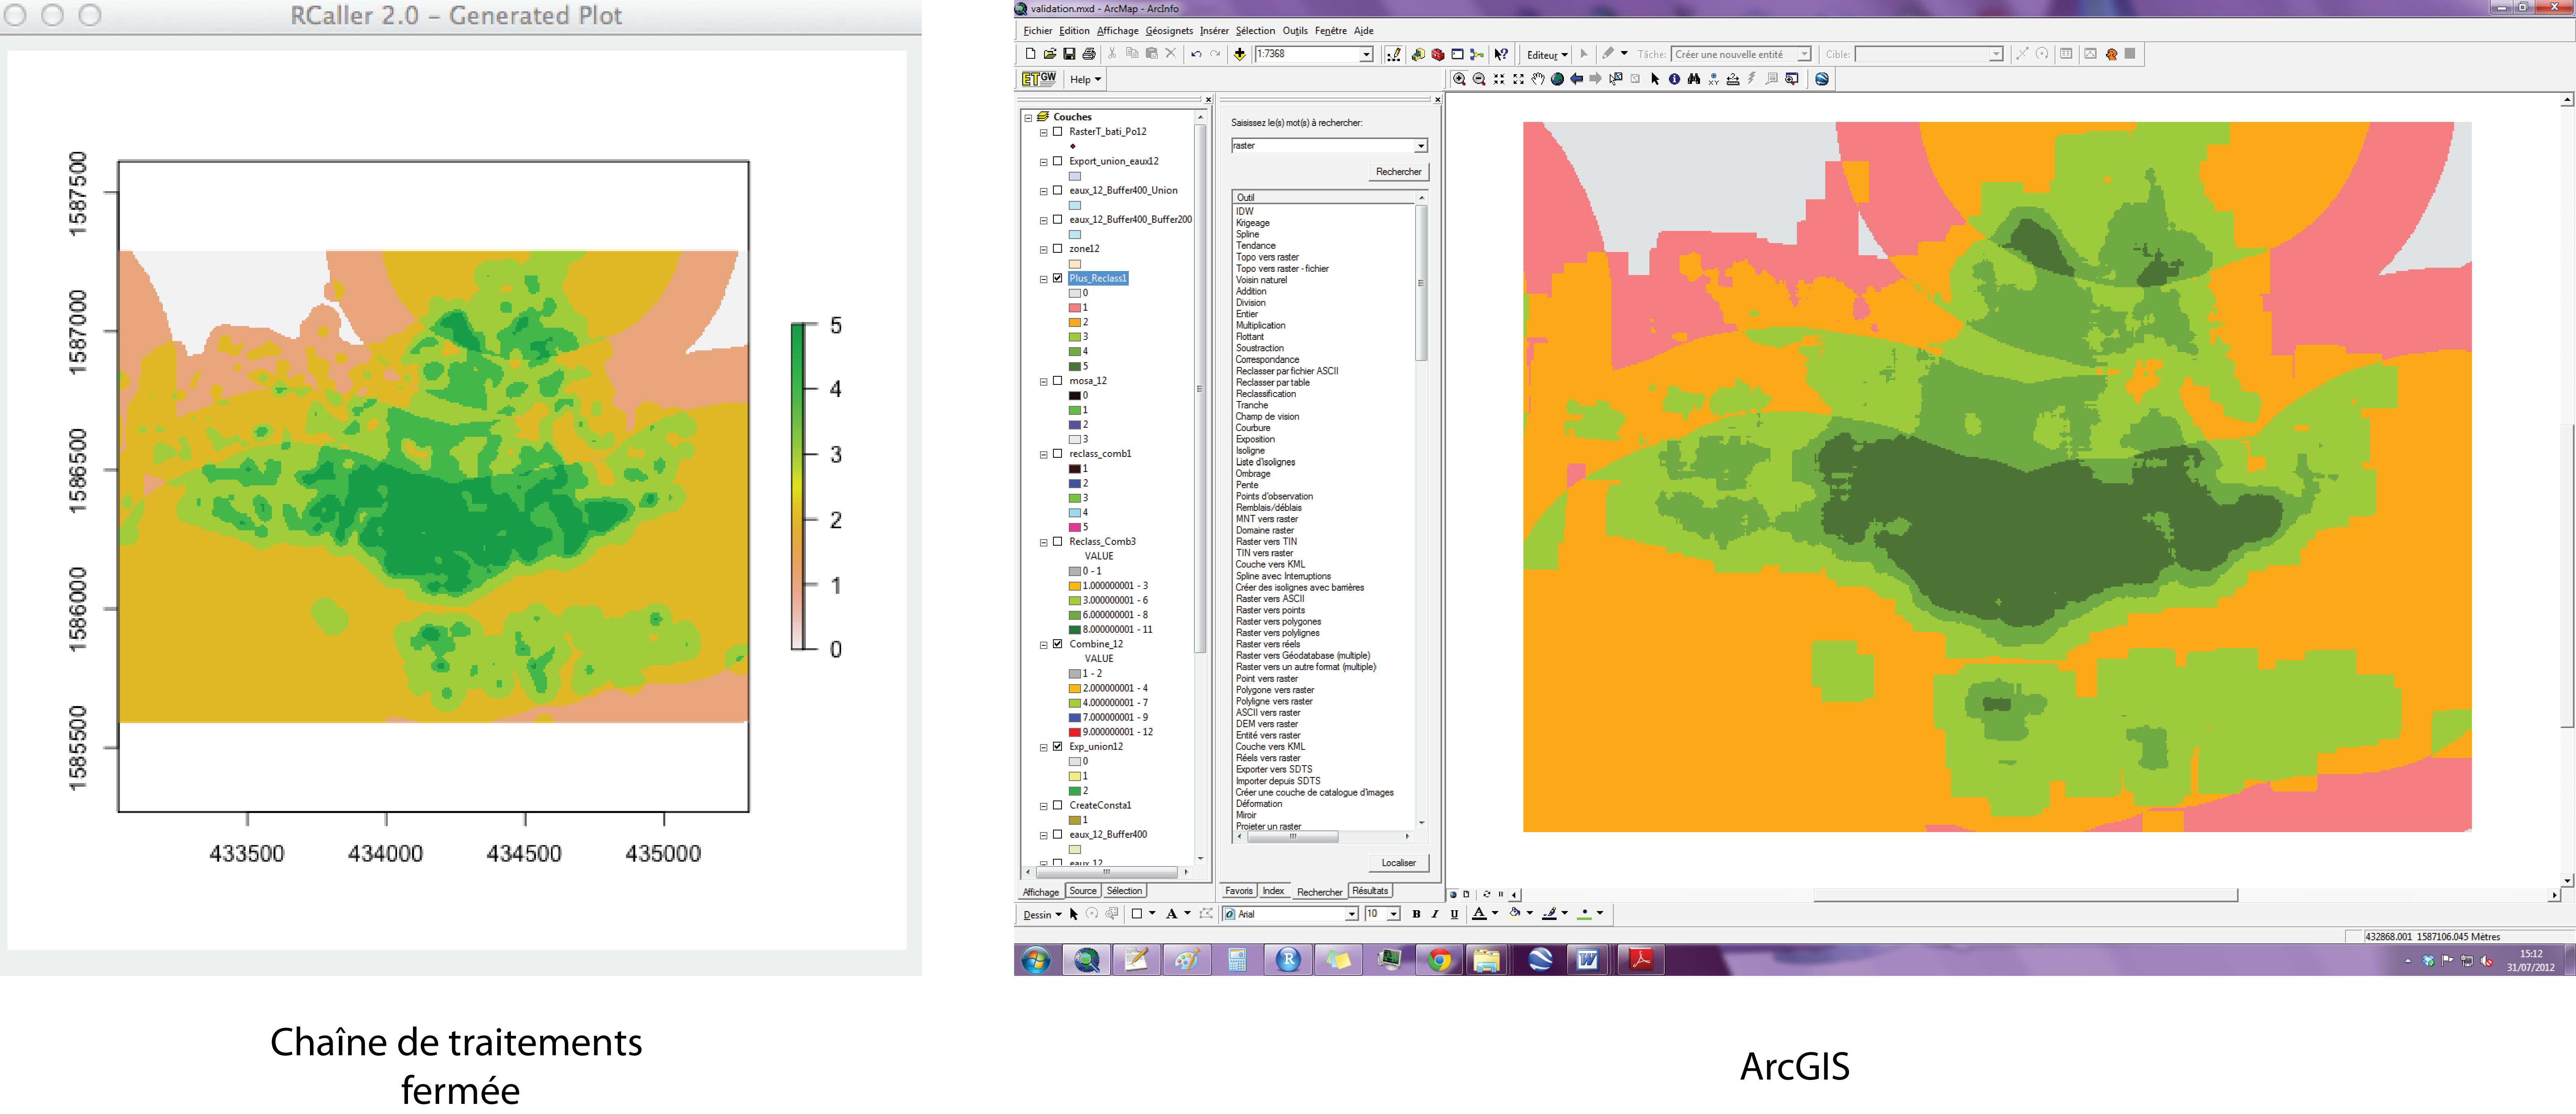
\includegraphics[width=14cm]{RisqueComp}\\
\caption{\label{RisqueComp} Cartes de risque}
\end{figure}
\end{center}

La carte de risque est obtenu est combinant la carte d'aléa et la carte de vulnérabilité. \\

Sous R, nous avons testé plusieurs possibilité pour effectuer ce genre d'opération. Nous avons obtenu le meilleur rendu en effectuons une addition des deux raster. Pour chaque pixel d'une image qui superpose avec un autre pixel d'une autre image, les valeurs des deux pixels sont additionnées.

Afin de valider cette approche, nous avons effectué la même opération sous ArcGIS. Les deux cartes valident nos résultats car ils sont à nouveau très similaires. 

\section{Difficultés rencontrées}

Tout au long du développement informatique de la chaîne de traitements et du logiciel ouvert, nous avons été confrontés à de nombreuses difficultés. Dans cette partie j'expliquerai les problèmes majeurs afin de faciliter le futur développement informatique de l'outil. Les difficultés sont regroupées en trois sous-parties : Difficultés liées au développement en Java, difficultés liées à l'utilisation de PostgreSQL / PostGIS et difficultés liées au logiciel R.\\

\subsection{Java}

Sur internet, il existe un nombre infini de forum et de tutoriels sur tout ce qui est programmation en Java. Ainsi, j'ai pu acquérir de nouvelles connaissances dans ce domaine. Néanmoins ce qui a été très compliqué, était de comprendre le fonctionnement de Rcaller, permettant d'utiliser les fonctionnalités de R sous Java. Il existe en effet que très peu de documentations et informations sur internet pour cette extension de Java. \\
La prise en main de Rcaller a nécessité un certain temps. Par exemple, nous avons dû faire face au problème que lors de l'affichage d'une donnée (plot), la fermeture d'une fenêtre causait automatiquement la fermeture de tout le programme. Pour résoudre ce problème, le résultat (l'image affichée) doit être stocké temporairement et par la suite être affiché dans une nouvelle fenêtre. \\
Une autre difficulté a été de comprendre comment intégrer des variables Java dans le code "R". Par exemple, en ce qui concerne la reclassification d'une image raster, l'utilisateur peut choisir le nombre de classes et les valeurs minimales et maximales de chaque classe. La commande "addDoubleArray" de RCaller permet d'intégrer un tableau composé de valeurs du type double dans le code R. En fonction des choix de l'utilisateur, Rcaller crée à l'intérieur du code R une "matrice" comportant les valeurs du tableau Java. \\

Il est également possible de récupérer les résultats de calculs effectués dans R. On peut seulement récupérer le résultat de la dernière ligne du code R. Par exemple, si on calcule deux moyennes différentes, il est nécessaire de stocker les deux moyennes dans une "liste" (moyenne <- list(moyenne1,moyenne2) sous R). Avec la commande "runAndReturnResult (moyenne)" il est par la suite possible de récupérer le résultat des calculs stocké dans la liste "moyenne".\\

Ces illustrations rendent compte très partiellement des nombreuses difficultés que nous avons rencontrées en utilisant RCaller. Finalement il faut aussi préciser que l'exécution de cette extension est en général très lente, notamment si l'utilisateur ne dispose pas d'une machine performante.

\subsection{PostgreSQL/PostGIS}

En ce qui concerne l'utilisation de PostGIS et de PostgreSQL, ce qui a été le plus compliqué était certainement l'installation. Lorsque nous avons démarré le développement informatique de la chaîne de traitements, nous utilisions une version antérieure de PostgreSQL et de PostGIS. Le 3 avril 2012 est sortie PostGIS 2.0 avec comme principale nouveauté la gestion des images rasters. Le passage à la nouvelle version a été assez compliqué, notamment sous le système d'exploitation Linux. En effet, toutes les librairies utilisées par PostGIS comme GDAL, PROJ etc. ont dû être mises à jour, tout comme la version de PostgreSQL (minimum 8.4). Sous Windows et MacOS ceci a posé moins de problèmes car des exécutables d'installation sont disponibles sur internet et les anciennes versions peuvent être supprimées plus facilement.\\

Souvent il n'est pas possible d'effectuer des opérations sur des données spatiales stockées dans la base de données, probablement parce qu'il y a eu un problème de type de géométrie lors de la construction de la donnée. Pour résoudre ce problème, il ést nécessaire pour chaque traitement PostGIS (par exemple Intersection entre deux couches) de créer une donnée "temporaire" à l'aide la fonctionnalité PostGIS "ST\_Buffer". Cette fonctionnalité crée théoriquement des zones tampons. En créant des zones de tampons de taille zéro, la fonctionnalité permet également de résoudre ce genre de problème.\\
% regarder les fonctions de détéction et transformation de types 


\subsection{R}

Par rapport à l'utilisation de R, nous avons été confronté à une difficulté majeure qui est l'utilisation de la librairie "rgdal". Sous Linux, il a été assez facile d'installer cette libraire à l'aide de la commande R "install.packages("rgdal")", néanmoins il est important de vérifier que lors de l'installation les versions de GDAL, PROJ et GEOS soient mises à jour car sinon un certain nombre de fonctionnalités risque de ne pas fonctionner. \\

Sous MacOS, il est nécessaire de faire l'installation à partir de la  source du package. Sur le site \url{http://www.r-bloggers.com/installing-rgdal-on-mac-os-x-2/} sont expliquées les informations nécessaires pour cette opération.\\

Sous Windows, l'installation de rgdal est facile et se fait à l'aide de la commande "install.packages". Malheureusement, il est impossible d'influencer la version GDAL utilisée lors de l'installation du package. Ainsi, il est actuellement impossible de charger des données dans R à partir d'une base de données PostgreSQL en utilisant rgdal. Ainsi, sous Windows, la chaîne de traitements ne fonctionne pas encore et le logiciel libre présente des fonctionnalités limitées (tous les traitements liés à l'utilisation de R ne fonctionnent pas).\\


\section{Perspectives}

L'objectif principal du stage était la conceptualisation et le développement informatique d'une chaîne de traitements permettant de cartographier le risque de transmission du paludisme. La définition des facteurs de risque de transmission du paludisme a été une première étape indispensable de ce travail.\\

Le modèle conceptuel ainsi que les listes concernant les différents facteurs de risque de transmission permettent aux experts, mais également à des non-experts, de comprendre les éléments  du cycle du paludisme et comment le paludisme se développe.\\

A partir de ce modèle conceptuel, nous avons pu définir les traitements nécessaires pour cartographier le risque. Par la suite,  de nombreuses réflexions autour de l'architecture informatique ont été menées. L'objectif était que la chaîne soit réutilisable pour le plus grand nombre de personnes. Créer un logiciel basé sur une architecture OpenSource et libre était donc indispensable. Nous avons décidé de développer la chaîne en Java. Par la suite, nous avons recherché pour chaque traitement les libraires et outils nécessaires. Très rapidement, nous nous sommes aperçus que PostgreSQL, PostGIS (traitements d'analyse spatiale) et R (notamment pour les traitements statistiques et les traitements raster) permettent d'effectuer tous les traitements que nous devions enchaîner.\\

Au bout de quatre mois, le développement informatique a abouti à une première chaîne de traitements fermée. Cette chaîne de traitements effectue un certain nombre de traitement dans un ordre bien précis, l'utilisateur n'a aucune influence sur le déroulement des traitements.\\

Avec les différents encadrants (et comme le travail avait avancé plus vite que prévu), nous avons décidé qu'il serait intéressant de développer, en se basant sur les traitements de la chaîne de traitements, un logiciel qui permettra d'effectuer chaque traitement indépendamment.\\

Le logiciel qui a été développé permet d'imaginer de nombreuses perspectives. A court terme, il peut être très intéressant de faire évaluer l'outil et de bien sûr rédiger un mode d'emploi pour l'outil et relever les retours des utilisateurs. D'ores et déjà, nous pensons qu'il serait bien  d'améliorer l'affichage des données (avec Grass par exemple) et d'améliorer la gestion des couches dans la base. La possibilité de se connecter à une base de données externe (hébergé sur un serveur internet) permet aussi d'envisager l'utilisation de l'outil dans de nombreux projets. Beaucoup de gens sont intéressés par les fonctionnalités de PostGIS, mais ne disposent pas des connaissances nécessaires pour son utilisation. Le logiciel leur permet dans un premier temps de créer une base de données, d'insérer des vecteurs et des rasters dans cette base et d'effectuer un certain nombre de traitements sur ces données. A long terme, l'intégration de nouveaux traitements pourrait faire de ce logiciel un outil précieux pour les gens souhaitant d'effectuer des traitements d'analyse spatiale de base (intersection, union, zones tampon etc.).

A long terme, il peut être envisagé de créer un équivalent du  "ModelBuilder" d'ArcGIS. L'utilisateur pourrait donc créer ses propres chaînes de traitements en fonction de ses besoins. En plus, il est alors envisageable que ces chaînes soient capitalisables et réutilisables.

\section{Conclusion}

Au terme des six mois de stage, la collaboration avec des experts dans des domaines divers (informatique, environnement, environnement-santé, biologie etc.) m'a permis d'acquérir un grand nombre de connaissances et de compétences et de travailler sur une multitude de thématiques.\\

L'élaboration d'un modèle conceptuel autour des éléments du paludisme a nécessité une recherche bibliographique importante ainsi qu'une longue phase de réflexion. Ce travail m'a donc surtout apporté beaucoup sur le plan scientifique.\\

Dans un deuxième temps, le développement respectivement d'une chaîne de traitements fermée et d'un logiciel ouvert m'a permis d'approfondir mes connaissances dans plusieurs domaines de l'informatique : Gestion des bases de données (spatiales), R et surtout programmation en Java sans oublier bien évidemment la conceptualisation et toutes les étapes de réflexion de la chaîne en amont.\\

Toutes les étapes, les erreurs et les leçons tirées de ce stage m'ont beaucoup aidé à évoluer dans le monde des SIG et plus particulièrement dans le domaine de l'informatique.\\

La qualité des résultats obtenus avec la chaîne de traitements fermée comparéé à celle des résultats obtenus à partir d'ArcGIS démontre les capacités des outils développés dans le cadre de ce travail et des outils et librairies libres et gratuites comme PostGIS/PostGreSQL et R. Les outils peuvent intéresser beaucoup de personnes, non seulement en ce qui concerne la cartographie de risques environnementaux, mais également pour effectuer des traitements d'analyse ou pour gérer et créer des bases de données spatiales. La possibilité de se connecter à une base de données distante est certainement un des atouts de cet outil.

Finalement, les objectifs du stage ont été atteints. La chaîne de traitements fermée est opérationnelle. Le logiciel ouvert permet, quant à lui, d'effectuer chacun des traitements de manière indépendante. 

